\documentclass[10pt,xcolor=pdflatex]{beamer}
\usepackage{newcent}
\usepackage[utf8]{inputenc}
\usepackage[czech]{babel}

\usepackage{hyperref} % \href for image (\includegraphics)
\usepackage{fancyvrb}
\usetheme{FIT}

\usepackage{soul} % for crossing text (\st{})

\definecolor{sourcesclr}{rgb}{.38,.38,.38}
\newcommand{\srctext}[1]{{\fontsize{7}{9}\selectfont\textcolor{sourcesclr}{#1}}}

\newenvironment<>{positiveblock}[1]{%
  \begin{actionenv}#2%
      \def\insertblocktitle{#1}%
      \par%
      \mode<presentation>{%
        \setbeamercolor{block title}{fg=white,bg=green!20!black}
       \setbeamercolor{block body}{fg=black,bg=green!40}
       \setbeamercolor{itemize item}{fg=green!20!black}
       \setbeamertemplate{itemize item}[triangle]
     }%
      \usebeamertemplate{block begin}}
    {\par\usebeamertemplate{block end}\end{actionenv}}

\newenvironment<>{negativeblock}[1]{%
  \begin{actionenv}#2%
      \def\insertblocktitle{#1}%
      \par%
      \mode<presentation>{%
        \setbeamercolor{block title}{fg=white,bg=red!20!black}
       \setbeamercolor{block body}{fg=black,bg=red!20}
       \setbeamercolor{itemize item}{fg=red!20!black}
       \setbeamertemplate{itemize item}[triangle]
     }%
      \usebeamertemplate{block begin}}
    {\par\usebeamertemplate{block end}\end{actionenv}}


%%%%%%%%%%%%%%%%%%%%%%%%%%%%%%%%%%%%%%%%%%%%%%%%%%%%%%%%%%%%%%%%%%
\title{Lego Mindstorm EV3 ve výuce programování a robotiky}

\author[]{Jaroslav Páral}

\institute[]{Vysokého učení technického v Brně, Fakulta informačních technologií\\
Bo\v{z}et\v{e}chova 1/2, 612 66 Brno - Kr\'alovo Pole\\
xparal02@stud.fit.vutbr.cz}

\date{13. června 2017}
%\date{\today}
%\date{} % bez data

%%%%%%%%%%%%%%%%%%%%%%%%%%%%%%%%%%%%%%%%%%%%%%%%%%%%%%%%%%%%%%%%%%

\begin{document}

\frame[plain]{\titlepage}


\begin{frame}\frametitle{Výukový roboti}
    \vspace{15mm}
    \begin{figure}[h]
    	\begin{minipage}[b]{.45\textwidth}
    		\centering
    		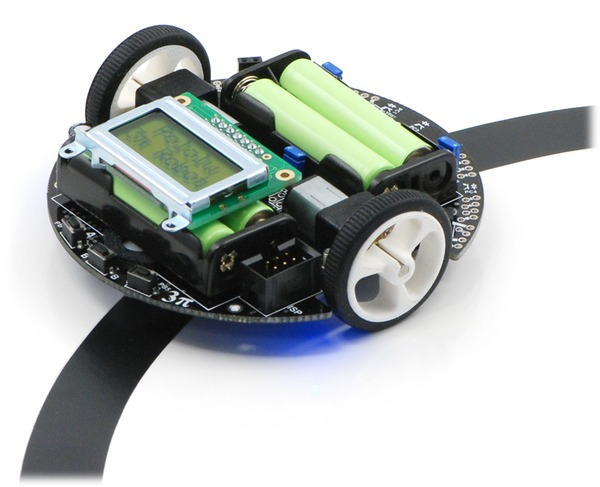
\includegraphics[width=\textwidth]{../text/images/pololu-3pi-robot-8-on-line.jpg}
    		%\caption[Robot Pololu 3pi]{Robot Pololu 3pi\protect\footnotemark}
    		\label{fig:pololu-3pi-robot-8-on-line}
    	\end{minipage}
    	\hfill
    	\begin{minipage}[b]{.45\textwidth}
    		\centering
    		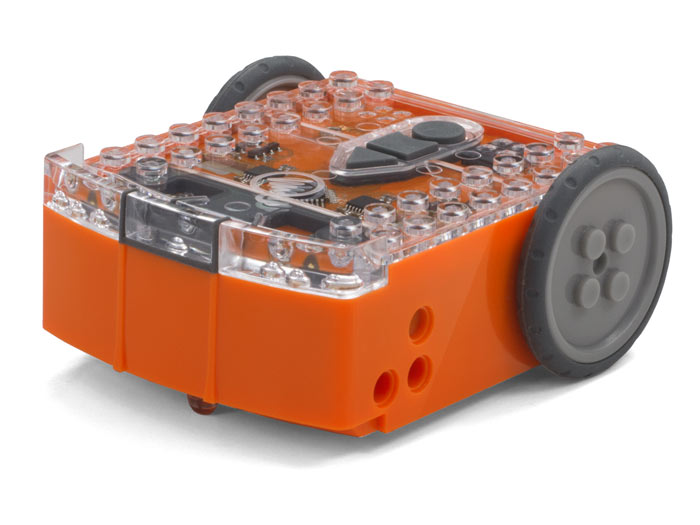
\includegraphics[width=\textwidth]{../text/images/Edison-Educational-robot.jpg}
    		%\caption[Robot Edison]{Robot Edison\protect\footnotemark}
    		\label{fig:Edison-Educational-robot}
    	\end{minipage}
    \end{figure}

    \vspace{15mm}
    \srctext{Zdroj levý obrázek: \url{https://www.pololu.com/product/975} \\}
    \srctext{Zdroj pravý obrázek: \url{https://meetedison.com/meet-edison-v2-0/}}
\end{frame}


\begin{frame}\frametitle{LEGO MINDSTORMS EV3}
    \begin{figure}[h]
    	\centering
    	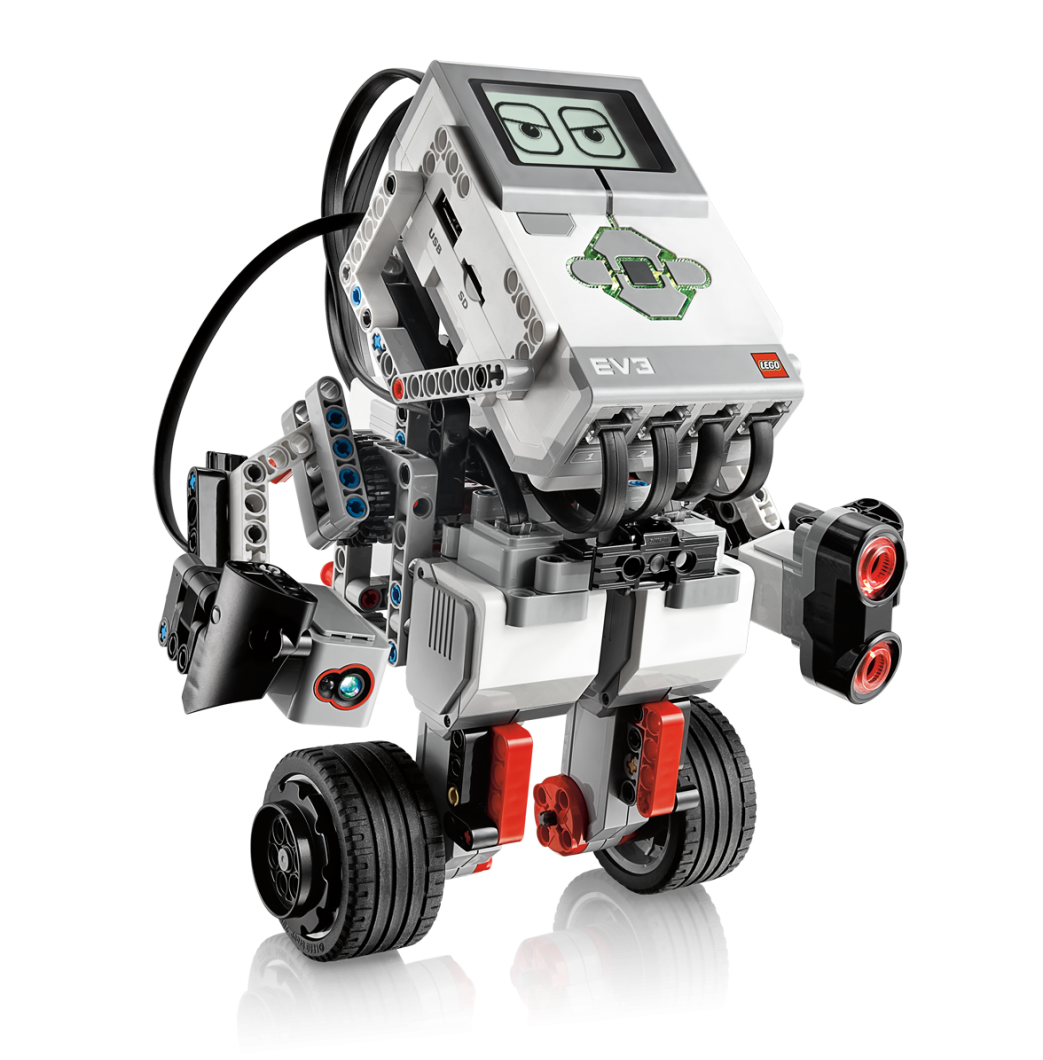
\includegraphics[width=190px]{img/lego-mindstorms-ev3_Robotics-for-Kids.png}
    	%\caption[\legoEV{ }-- samobalancující robot]{\legoEV{ }-- balancující robot\protect\footnotemark}
    	\label{fig:lego-mindstorms-ev3_Robotics-for-Kids}
    \end{figure}

    \srctext{Zdroj obrázek: \url{https://www.bermotech.com/training/coding-for-teenagers-and-children/y-robotics-with-lego-mindstorm-ev3/}}
\end{frame}


\begin{frame}\frametitle{Originální vývojové prostředí pro LEGO}
    \begin{columns}
        \column{.48\textwidth}
            \begin{positiveblock}{Výhody}
                \begin{itemize}
                    \item jednoduché rozhraní
                    \item intuitivní používání
                    \item vhodné "od 7 let"
                \end{itemize}
            \end{positiveblock}
        
        \column{.48\textwidth}
    \end{columns}
            
    \vspace{10mm}
    \begin{figure}[h]
   	    \centering
  	     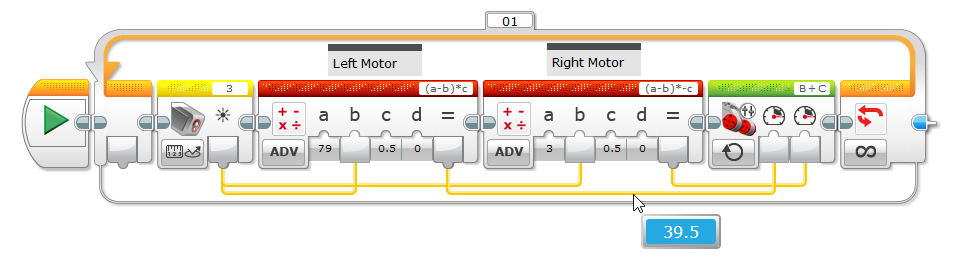
\includegraphics[width=\textwidth]{../text/images/lego-soft_live-debugging_line-advance.png}
    \end{figure}  
\end{frame}


\begin{frame}\frametitle{Originální vývojové prostředí pro LEGO}
    \begin{columns}
        \column{.48\textwidth}
            \begin{positiveblock}{Výhody}
                \begin{itemize}
                    \item jednoduché rozhraní
                    \item intuitivní používání
                    \item vhodné "od 7 let"
                \end{itemize}
            \end{positiveblock}
        
        \column{.48\textwidth}
            \begin{negativeblock}{Problémy}
                \begin{itemize}
                    \item rozsáhlé programy
                    \item pokročilé úpravy
                    \item orientace
                \end{itemize}
            \end{negativeblock}
    \end{columns}
            
    \vspace{7mm}
    \begin{figure}[h]
   	    \centering
  	     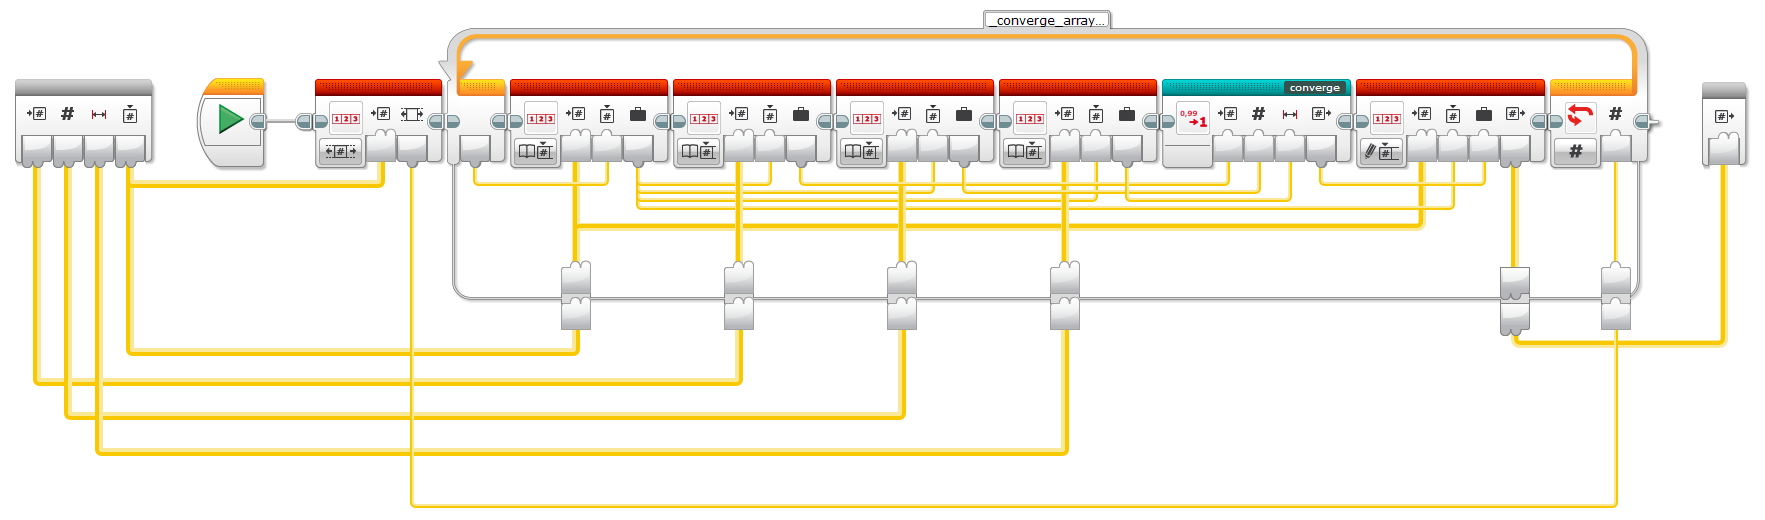
\includegraphics[width=\textwidth]{../text/images/lego-soft_legolib_converge_array.png}
   	    %\caption[Ukázka nepřehlednosti rozsáhlejších programů]{Ukázka nepřehlednosti rozsáhlejších programů - žluté dráhy značí předávání vstupních a~výstupních parametrů mezi jednotlivými bloky - velmi špatně se zjišťuje a~kontroluje správnost zapojení žlutých drah.}
   	    \label{fig:lego-soft_legolib_converge_array}
    \end{figure}  
\end{frame}


\begin{frame}\frametitle{Systém EV3RT}
    \large
    \begin{columns}
        \column{.48\textwidth}
             Vlastnosti:
            \begin{itemize}
                \item RTOS
                \item open-source
                \item multiplatformní
                \item až o 3 řády výkonnější
            \end{itemize}
        
        \pause
        
        \column{.48\textwidth}
            Připravil jsem:
            \begin{itemize}
                \item C++ API 
                \pause      
                \item vývojové prostředí        
                \pause 
                \item dokumentaci        
                \pause
                \item ukázkové příklady % tutoriály
            \end{itemize}

    \end{columns}
\end{frame}


\begin{frame}\frametitle{C++ API}
    \centering
    \large
    Cíl: Usnadnit přechod ze standardního vývojového prostředí.

    \vspace{10mm}
    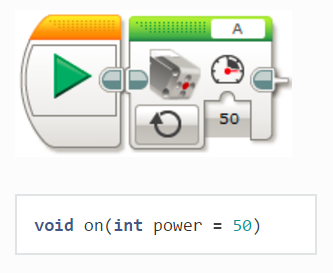
\includegraphics[width=140px]{img/doc-motor_on.png}
\end{frame}


\begin{frame}\frametitle{Vývojové prostředí}
    \centering
    \large
    Visual Studio Code
    \begin{figure}[h]
      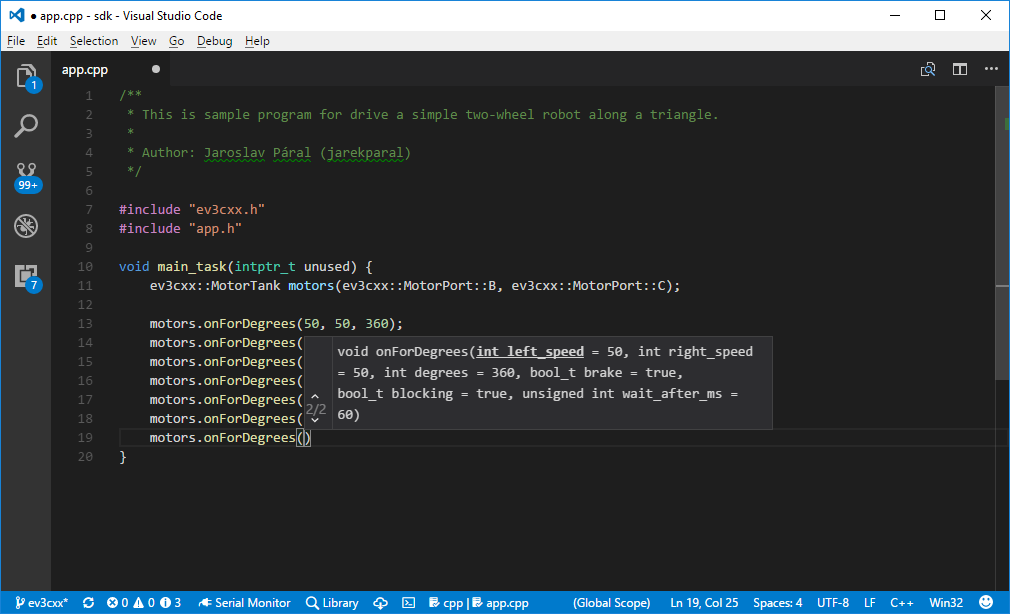
\includegraphics[width=\textwidth]{../text/images/visual-studio-code_intellisense-param.png}
    \end{figure}
\end{frame}


\begin{frame}\frametitle{Dokumentace}
    \vspace{-5mm}
    \begin{figure}[h]
    	\centering
    	\href{http://rb3rt.readthedocs.io/cs/latest/ev3cxx\_motor-class.html\#onforseconds}{
            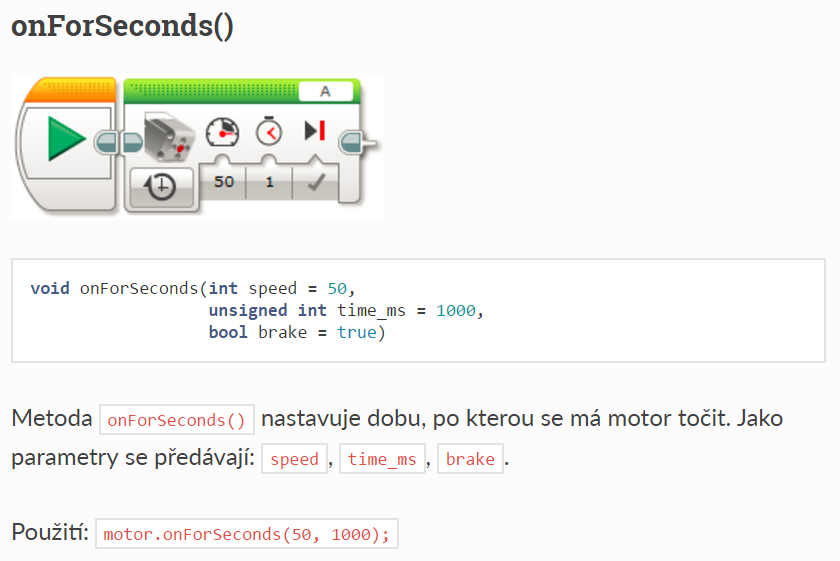
\includegraphics[width=320px]{img/web-documentation.png}
        }
    \end{figure}

\end{frame}


\begin{frame}\frametitle{Závěr}
    \begin{columns}
        \column{.48\textwidth}
            \begin{itemize}
                \item výkonnostní testy 
                \item C++ API    
                \item vývojové prostředí        
                \item dokumentaci        
                \item ukázkové příklady % tutoriály
                \item prakticky využíváno
            \end{itemize}
    
        \pause
        
        \column{.48\textwidth}
            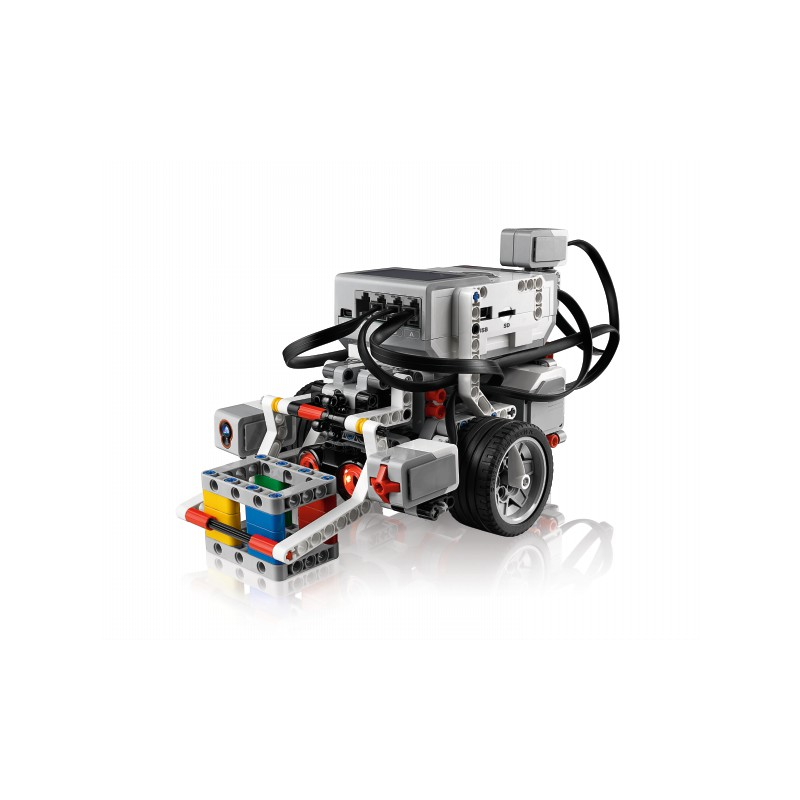
\includegraphics[width=120px]{img/lego-mindstorms-ev3-education-kit-with-software.JPG}
    \end{columns}

    
    \centering
    \vspace{10mm}
    \large
    Děkuji Vám za pozornost.

    \vspace{10mm}
    \small
    Dokumentace k projektu: \url{http://rb3rt.readthedocs.io}

    \vspace{10mm}
    \raggedright
    \srctext{Zdroj obrázek: \url{https://www.generationrobots.com/en/402314-lego-mindstorms-ev3-education-kit-with-software.html}}
\end{frame}


\begin{frame}\frametitle{Otázka od oponenta}
    \centering
    \large
    Otázka:\\
    V práci zmiňujete práci se studenty. Konzultoval jste postup či podobu také s pedagogy?

    \vspace{10mm}
    Odpověď:\\
    Konzultoval jsem postup s lektory z Robotárny (Dům dětí a mládeže Brno, Helceletova), kteří již několik let vedou kroužky s LEGO MINDSTORMS.

\end{frame}


\begin{frame}\frametitle{Ukázkový příklad}
    \centering
    {
        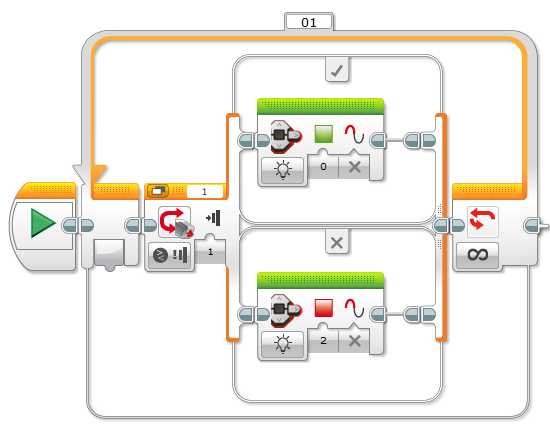
\includegraphics[width=\textwidth]{img/ev3cxx_robotutorial_05-switch.png}
    }
\end{frame}


\begin{frame}\frametitle{Ukázkový příklad}
    \centering
    \href{http://rb3rt.readthedocs.io/cs/latest/ev3cxx_robotutorial/05-switch.html}{
        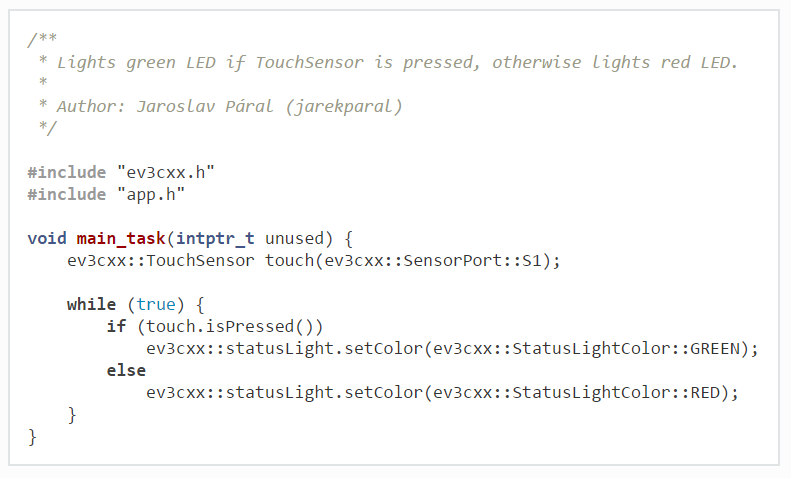
\includegraphics[width=\textwidth]{img/ev3cxx_robotutorial_05-switch_source-code.png}
    }
\end{frame}

% \bluepage{Thank You For Your Attention !}

\end{document}





\begin{frame}\frametitle{Závěr}
    Připravil jsem:
    \begin{itemize}
        \item C++ API 
        \item vývojové prostředí        
        \item dokumentaci        
        \item ukázkové příklady % tutoriály
    \end{itemize}    
    \pause
    
    \centering
    \vspace{10mm}
    \large
    Děkuji Vám za pozornost.

    \vspace{10mm}
    \small
    Dokumentace k projektu: \url{http://rb3rt.readthedocs.io}

\end{frame}



\begin{frame}\frametitle{Systém EV3RT}
    Vlastnosti:
    \begin{itemize}
        \item RTOS
        \item open-source
        \item multiplatformní
        \item o 2 až 3 řády výkonnější
    \end{itemize}
\end{frame}



\begin{frame}\frametitle{Alternativní prostředí}
    \begin{columns}
        \column{.48\textwidth}
            \begin{positiveblock}{Prostředí}
                \begin{itemize}
                    \item ROS
                    \item Matlab/LabVIEW
                    \item ROBOTC
                    \item {\it ev3dev}
                    \item EV3RT
                \end{itemize}
            \end{positiveblock}
        
        \column{.48\textwidth}
            \begin{negativeblock}{Požadavky}
                \begin{itemize}
                    \item 
                    \item 
                    \item 
                    \item 
                    \item 
                \end{itemize}
            \end{negativeblock}
    \end{columns}
\end{frame}

\begin{frame}\frametitle{Alternativní prostředí}
    \begin{columns}
        \column{.48\textwidth}
            \begin{positiveblock}{Prostředí}
                \begin{itemize}
                    \item \st{ROS}
                    \item Matlab/LabVIEW
                    \item ROBOTC
                    \item {\it ev3dev}
                    \item EV3RT
                \end{itemize}
            \end{positiveblock}
        
        \column{.48\textwidth}
            \begin{negativeblock}{Požadavky}
                \begin{itemize}
                    \item nezávislé na PC
                    \item 
                    \item 
                    \item 
                    \item 
                \end{itemize}
            \end{negativeblock}
    \end{columns}
\end{frame}

\begin{frame}\frametitle{Alternativní prostředí}
    \begin{columns}
        \column{.48\textwidth}
            \begin{positiveblock}{Prostředí}
                \begin{itemize}
                    \item \st{ROS}
                    \item \st{Matlab/LabVIEW}
                    \item \st{ROBOTC}
                    \item {\it ev3dev}
                    \item EV3RT
                \end{itemize}
            \end{positiveblock}
        
        \column{.48\textwidth}
            \begin{negativeblock}{Požadavky}
                \begin{itemize}
                    \item nezávislé na PC
                    \item licenční poplatky
                    \item multiplatformní
                    \item 
                    \item 
                \end{itemize}
            \end{negativeblock}
    \end{columns}
\end{frame}

\begin{frame}\frametitle{Alternativní prostředí}
    \begin{columns}
        \column{.48\textwidth}
            \begin{positiveblock}{Prostředí}
                \begin{itemize}
                    \item \st{ROS}
                    \item \st{Matlab/LabVIEW}
                    \item \st{ROBOTC}
                    \item \st{{ev3dev}}
                    \item EV3RT
                \end{itemize}
            \end{positiveblock}
        
        \column{.48\textwidth}
            \begin{negativeblock}{Požadavky}
                \begin{itemize}
                    \item nezávislé na PC
                    \item licenční poplatky
                    \item multiplatformní
                    \item výkon
                    \item real-time běh
                \end{itemize}
            \end{negativeblock}
    \end{columns}
\end{frame}
